\documentclass{article}
\usepackage{fancyhdr} % for pretty formatting
\usepackage{amsmath} % for matrices
\usepackage{amssymb} % for bold text
\usepackage{pgfplots} % for graphs
\usepackage{hyperref} % for hyperlinks
\pgfplotsset{compat=1.18}
\usepackage{enumitem} % for custom lists

\usepackage{lipsum} % For dummy text
\usepackage{cite} % For citations

\pagestyle{fancy}  
\fancyhf{} % Clear all header and footer fields

\usepackage{tcolorbox} % Required for tcolorbox

\newtcolorbox{solutioncheck}{
    colback=green!10, % Background color
    colframe=gray!50, % Frame color
    boxsep=5pt, % Padding
    arc=4pt, % Rounded corners
    title=Checking solution, % Optional title for the aside
    fonttitle=\bfseries, % Title font style
} % for Asides

\lhead{Joshua Dunne}
\rhead{\thepage} % Displays the current page number 
\lfoot{MATH620}
\rfoot{Unit 3}
\cfoot{Homework 4}

\begin{document}
\section{Question 1}
    \paragraph{Given}
        We are given three different vectors to try to map through a
        given function. We are then to plot everything.
        \begin{enumerate}
            \item $\mathbf{A} = \begin{bmatrix}3 & 0\\0 & -2\end{bmatrix}$
            \item $T: \mathbb{R}^2 \rightarrow \mathbb{R}^2 $ 
            \item$T(\mathbf{x})=\mathbf{A}\mathbf{x}$
        \end{enumerate}
    \paragraph{Find}
        \begin{enumerate}
            \item 
                The image of $u$ under $T$ where
                $\mathbf{u} = \begin{bmatrix}3\\-1\end{bmatrix}$
            \item 
                The image of $c$ under $T$ where
                $\mathbf{v} = \begin{bmatrix}0\\1.5\end{bmatrix}$
            \item The image of $\mathbf{u} + \mathbf{v}$
        \end{enumerate}
    \subsection{Work}
        \paragraph{Images}
            The image under is just going to be the result of having the function
            applied. We can do as such like so, for each of the given terms
            \begin{enumerate}
                \item 
                    $T(\mathbf{u}) = A\mathbf{u} = \begin{bmatrix}3 & 0\\0 & -2\end{bmatrix}\begin{bmatrix}3\\-1\end{bmatrix} = \begin{bmatrix}9\\2\end{bmatrix}$
                \item 
                    $T(\mathbf{v}) = A\mathbf{v} = \begin{bmatrix}3 & 0\\0 & -2\end{bmatrix}\begin{bmatrix}0\\1.5\end{bmatrix} = \begin{bmatrix}0\\-3\end{bmatrix}$
                \item 
                    $T(\mathbf{u}+\mathbf{v}) = A(\mathbf{u}+\mathbf{v}) = \begin{bmatrix}3 & 0\\0 & -2\end{bmatrix}\begin{bmatrix}0\\1.5\end{bmatrix} = \begin{bmatrix}9\\-1\end{bmatrix}$
            \end{enumerate}
    \newpage
    \subsection{Illustration}
        \paragraph{Scaling}
            Throughout we should expect to see a few things. The origin
            should remain constant, and relationships about perpendicularity
            and being parallel should contiue to hold.
        \begin{figure}[h!]
            \begin{center}
            \begin{minipage}[b]{0.4\textwidth}
                

            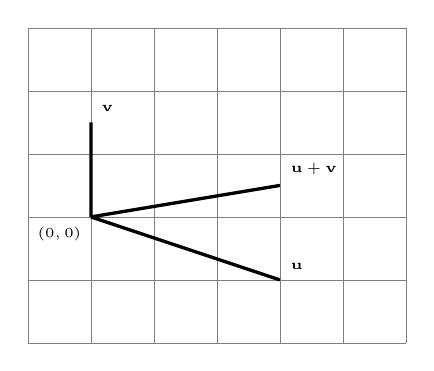
\begin{tikzpicture}[
                    every node/.style={font=\tiny},
                    scale=0.8 % Adjusted scale to fit a reasonable paper size, you can change this
                ]
                
                \draw[step=1.0, gray, very thin] (-1, -2) grid (5, 3);
                \node[below left] at (0,0) {$(0,0)$};
                \draw[very thick]
                    (0, 0) -- (3, -1) node[above right] {$\mathbf{u}$}
                    (0, 0) -- (0, 1.5) node[above right] {$\mathbf{v}$}
                    (0, 0) -- (3, .5) node[above right] {$\mathbf{u} + \mathbf{v}$};
                ;
            \end{tikzpicture}

            
            \end{minipage}
            \hspace{0.5cm}
            \begin{minipage}[b]{0.44\textwidth}
                

            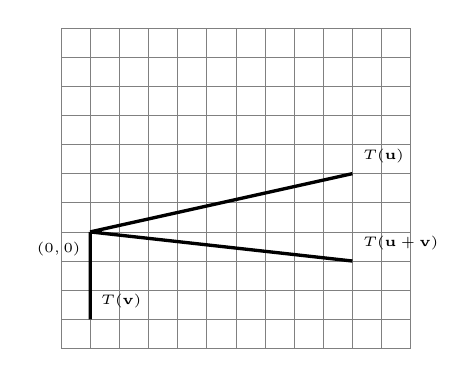
\begin{tikzpicture}[
                    every node/.style={font=\tiny},
                    scale=0.37 % Adjusted scale to fit a reasonable paper size, you can change this
                ]
                
                \draw[step=1.0, gray, very thin] (-1, -4) grid (11, 7);
                \node[below left] at (0,0) {$(0,0)$};
                \draw[very thick]
                    (0, 0) -- (9, 2) node[above right] {$T(\mathbf{u})$}
                    (0, 0) -- (0, -3) node[above right] {$T(\mathbf{v})$}
                    (0, 0) -- (9, -1) node[above right] {$T(\mathbf{u}+\mathbf{v})$};
                ;
            \end{tikzpicture}

             
            \end{minipage} 
            \end{center}
        \end{figure}
    
    \section{Question 2}
        \paragraph{Given}
            the matrix $A$:
            $$
                A = \begin{bmatrix} 1 & -5 & -7 \\ -3 & 7 & 5 \end{bmatrix}
            $$
            Define the linear transformation $T: \mathbb{R}^3 \rightarrow \mathbb{R}^2$ by $T(\mathbf{x}) = A\mathbf{x}$.
        \subsection{Prompts}
            \begin{enumerate}[label=(\alph*)]
                \item 
                    Find the image under T of $\mathbf{u}=\begin{bmatrix}2\\1\\-1\end{bmatrix}$
                    So. We have a 2x3 and we're multiplying by a 3x1. The result is going to be a 2x1
                    \begin{solutioncheck}
                        \[
                        \begin{bmatrix} 1 & -5 & -7 \\ -3 & 7 & 5 \end{bmatrix}
                        \begin{bmatrix}2\\1\\-1\end{bmatrix}
                        =
                        \begin{bmatrix}4\\-4\end{bmatrix}
                        \]
                    \end{solutioncheck}
                \item
                    Find a vector $\mathbf{x}$ whose image under
                    T is $\mathbf{b}=\begin{bmatrix}-12\\12\end{bmatrix}$
                    \paragraph{Thinking}
                        We can se up the system of equations so that we're solving for this.
                        As long as the solution $y\in\text{span}\{\mathbf{u},\mathbf{v}\}$
                    \paragraph{Solution}
                        \[
                        \begin{bmatrix} 1 & -5 & -7 \\ -3 & 7 & 5 \end{bmatrix}
                        \begin{bmatrix}x_1\\x_2\\x_3\end{bmatrix}
                        =
                        \begin{bmatrix}-12\\12\end{bmatrix}
                        \]
                        \begin{align*}
                            x_1 - 5x_2 - 7x_3 &= -12 \\
                            -3x_1 + 7x_2 + 5x_3 &= 12
                        \end{align*}
                        \begin{align*}
                            x_1 + 3x_3 &= 3 \\
                            x_2 + 2x_3 &= 3
                        \end{align*}
                        \subparagraph{Particular solution}
                            Let $x_3=0$ then $x_1=3$ and $x_2=3$.
                        \begin{solutioncheck}
                            \[
                            \begin{bmatrix} 1 & -5 & -7 \\ -3 & 7 & 5 \end{bmatrix}
                            \begin{bmatrix}3\\3\\0\end{bmatrix}
                            =
                            \begin{bmatrix}-12\\12\end{bmatrix}
                            \]
                        \end{solutioncheck}



            \end{enumerate}   

 
\end{document}